% Options for packages loaded elsewhere
\PassOptionsToPackage{unicode}{hyperref}
\PassOptionsToPackage{hyphens}{url}
%
\documentclass[
  ignorenonframetext,
]{beamer}
\usepackage{pgfpages}
\setbeamertemplate{caption}[numbered]
\setbeamertemplate{caption label separator}{: }
\setbeamercolor{caption name}{fg=normal text.fg}
\beamertemplatenavigationsymbolsempty
% Prevent slide breaks in the middle of a paragraph
\widowpenalties 1 10000
\raggedbottom
\setbeamertemplate{part page}{
  \centering
  \begin{beamercolorbox}[sep=16pt,center]{part title}
    \usebeamerfont{part title}\insertpart\par
  \end{beamercolorbox}
}
\setbeamertemplate{section page}{
  \centering
  \begin{beamercolorbox}[sep=12pt,center]{part title}
    \usebeamerfont{section title}\insertsection\par
  \end{beamercolorbox}
}
\setbeamertemplate{subsection page}{
  \centering
  \begin{beamercolorbox}[sep=8pt,center]{part title}
    \usebeamerfont{subsection title}\insertsubsection\par
  \end{beamercolorbox}
}
\AtBeginPart{
  \frame{\partpage}
}
\AtBeginSection{
  \ifbibliography
  \else
    \frame{\sectionpage}
  \fi
}
\AtBeginSubsection{
  \frame{\subsectionpage}
}

\usepackage{amsmath,amssymb}
\usepackage{lmodern}
\usepackage{iftex}
\ifPDFTeX
  \usepackage[T1]{fontenc}
  \usepackage[utf8]{inputenc}
  \usepackage{textcomp} % provide euro and other symbols
\else % if luatex or xetex
  \usepackage{unicode-math}
  \defaultfontfeatures{Scale=MatchLowercase}
  \defaultfontfeatures[\rmfamily]{Ligatures=TeX,Scale=1}
\fi
% Use upquote if available, for straight quotes in verbatim environments
\IfFileExists{upquote.sty}{\usepackage{upquote}}{}
\IfFileExists{microtype.sty}{% use microtype if available
  \usepackage[]{microtype}
  \UseMicrotypeSet[protrusion]{basicmath} % disable protrusion for tt fonts
}{}
\makeatletter
\@ifundefined{KOMAClassName}{% if non-KOMA class
  \IfFileExists{parskip.sty}{%
    \usepackage{parskip}
  }{% else
    \setlength{\parindent}{0pt}
    \setlength{\parskip}{6pt plus 2pt minus 1pt}}
}{% if KOMA class
  \KOMAoptions{parskip=half}}
\makeatother
\usepackage{xcolor}
\newif\ifbibliography
\setlength{\emergencystretch}{3em} % prevent overfull lines
\setcounter{secnumdepth}{-\maxdimen} % remove section numbering


\providecommand{\tightlist}{%
  \setlength{\itemsep}{0pt}\setlength{\parskip}{0pt}}\usepackage{longtable,booktabs,array}
\usepackage{calc} % for calculating minipage widths
\usepackage{caption}
% Make caption package work with longtable
\makeatletter
\def\fnum@table{\tablename~\thetable}
\makeatother
\usepackage{graphicx}
\makeatletter
\def\maxwidth{\ifdim\Gin@nat@width>\linewidth\linewidth\else\Gin@nat@width\fi}
\def\maxheight{\ifdim\Gin@nat@height>\textheight\textheight\else\Gin@nat@height\fi}
\makeatother
% Scale images if necessary, so that they will not overflow the page
% margins by default, and it is still possible to overwrite the defaults
% using explicit options in \includegraphics[width, height, ...]{}
\setkeys{Gin}{width=\maxwidth,height=\maxheight,keepaspectratio}
% Set default figure placement to htbp
\makeatletter
\def\fps@figure{htbp}
\makeatother

\makeatletter
\makeatother
\makeatletter
\makeatother
\makeatletter
\@ifpackageloaded{caption}{}{\usepackage{caption}}
\AtBeginDocument{%
\ifdefined\contentsname
  \renewcommand*\contentsname{Table of contents}
\else
  \newcommand\contentsname{Table of contents}
\fi
\ifdefined\listfigurename
  \renewcommand*\listfigurename{List of Figures}
\else
  \newcommand\listfigurename{List of Figures}
\fi
\ifdefined\listtablename
  \renewcommand*\listtablename{List of Tables}
\else
  \newcommand\listtablename{List of Tables}
\fi
\ifdefined\figurename
  \renewcommand*\figurename{Figure}
\else
  \newcommand\figurename{Figure}
\fi
\ifdefined\tablename
  \renewcommand*\tablename{Table}
\else
  \newcommand\tablename{Table}
\fi
}
\@ifpackageloaded{float}{}{\usepackage{float}}
\floatstyle{ruled}
\@ifundefined{c@chapter}{\newfloat{codelisting}{h}{lop}}{\newfloat{codelisting}{h}{lop}[chapter]}
\floatname{codelisting}{Listing}
\newcommand*\listoflistings{\listof{codelisting}{List of Listings}}
\makeatother
\makeatletter
\@ifpackageloaded{caption}{}{\usepackage{caption}}
\@ifpackageloaded{subcaption}{}{\usepackage{subcaption}}
\makeatother
\makeatletter
\@ifpackageloaded{tcolorbox}{}{\usepackage[many]{tcolorbox}}
\makeatother
\makeatletter
\@ifundefined{shadecolor}{\definecolor{shadecolor}{rgb}{.97, .97, .97}}
\makeatother
\makeatletter
\@ifpackageloaded{sidenotes}{}{\usepackage{sidenotes}}
\@ifpackageloaded{marginnote}{}{\usepackage{marginnote}}
\makeatother
\makeatletter
\makeatother
\ifLuaTeX
  \usepackage{selnolig}  % disable illegal ligatures
\fi
\IfFileExists{bookmark.sty}{\usepackage{bookmark}}{\usepackage{hyperref}}
\IfFileExists{xurl.sty}{\usepackage{xurl}}{} % add URL line breaks if available
\urlstyle{same} % disable monospaced font for URLs
\hypersetup{
  pdftitle={Investigation of direct and global downward sort-wave radiation over Thessaloniki},
  pdfauthor={Athanasios Natsis},
  hidelinks,
  pdfcreator={LaTeX via pandoc}}

\title{Investigation of direct and global downward sort-wave radiation
over Thessaloniki}
\subtitle{Includes newest trends!}
\author{Athanasios Natsis}
\date{2023-01-18}
\logo{\includegraphics{images/LAP3\_t\_bg.png}}

\begin{document}
\frame{\titlepage}
\ifdefined\Shaded\renewenvironment{Shaded}{\begin{tcolorbox}[boxrule=0pt, interior hidden, sharp corners, borderline west={3pt}{0pt}{shadecolor}, enhanced, breakable, frame hidden]}{\end{tcolorbox}}\fi

\begin{frame}{What we measure}
\protect\hypertarget{what-we-measure}{}
\end{frame}

\begin{frame}{How we measure}
\protect\hypertarget{how-we-measure}{}
\end{frame}

\begin{frame}{How we prosses}
\protect\hypertarget{how-we-prosses}{}
\end{frame}

\begin{frame}{Rusults}
\protect\hypertarget{rusults}{}
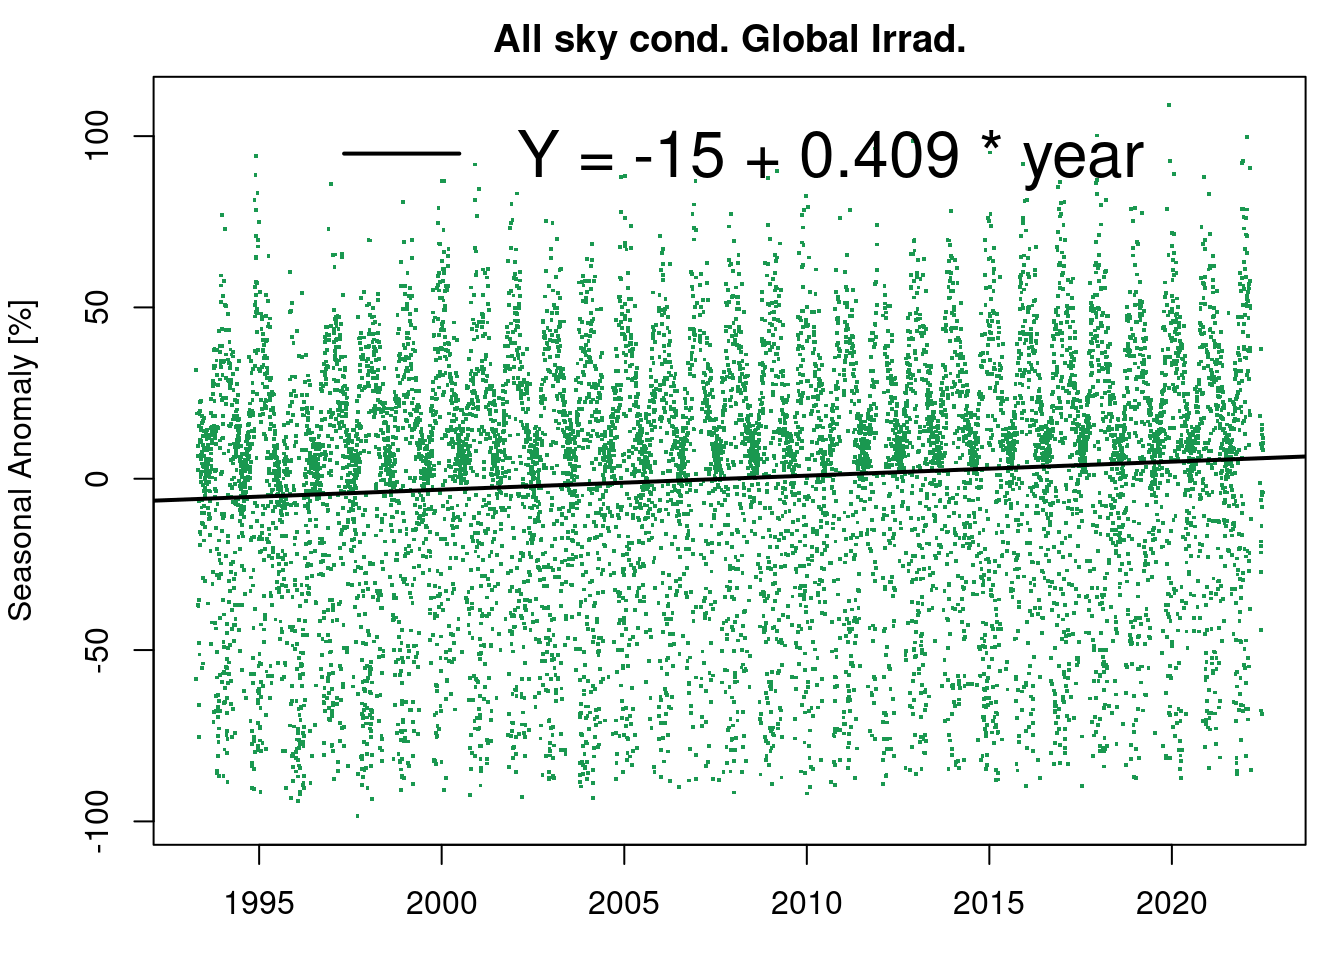
\includegraphics{images/DHI_GHI_1_longterm_trends_files/figure-html/longtermtrendsALL-4.pdf}
\end{frame}

\begin{frame}{3}
\protect\hypertarget{section}{}
\end{frame}

\begin{frame}{d}
\protect\hypertarget{d}{}
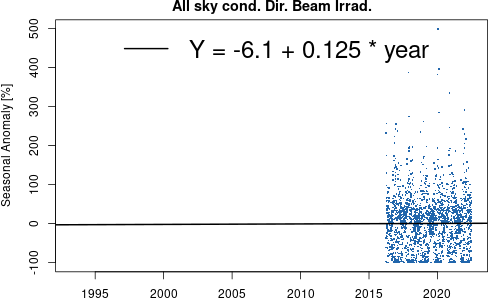
\includegraphics{images/DHI_GHI_1_longterm_trends_files/figure-html/longtermtrendsALL-3.png}
\end{frame}

\begin{frame}{d}
\protect\hypertarget{d-1}{}
\end{frame}

\begin{frame}{d}
\protect\hypertarget{d-2}{}
\end{frame}

\begin{frame}{d}
\protect\hypertarget{d-3}{}
\end{frame}

\begin{frame}{ddd}
\protect\hypertarget{ddd}{}
table of pers
\end{frame}

\begin{frame}{4}
\protect\hypertarget{section-1}{}
\end{frame}

\begin{frame}{5}
\protect\hypertarget{section-2}{}
\begin{columns}[T]
\begin{column}{0.5\textwidth}
\end{column}

\begin{column}{0.5\textwidth}
\end{column}
\end{columns}
\end{frame}

\begin{frame}{dddd}
\protect\hypertarget{dddd}{}
\begin{figure}

\begin{minipage}[t]{0.50\linewidth}

{\centering 

}

\end{minipage}%
%
\begin{minipage}[t]{0.50\linewidth}

{\centering 

}

\end{minipage}%
\newline
\begin{minipage}[t]{0.50\linewidth}

{\centering 

}

\end{minipage}%
%
\begin{minipage}[t]{0.50\linewidth}

{\centering 

}

\end{minipage}%

\end{figure}
\end{frame}

\begin{frame}{END}
\protect\hypertarget{end}{}
Quarto enables you to weave together content and executable code into a
finished presentation. To learn more about Quarto presentations see
\url{https://quarto.org/docs/presentations/}.
\end{frame}

\begin{frame}{Bullets}
\protect\hypertarget{bullets}{}
When you click the \textbf{Render} button a document will be generated
that includes:

\begin{itemize}
\tightlist
\item
  Content authored with markdown
\item
  Output from executable code
\end{itemize}
\end{frame}

\begin{frame}[fragile]{Code}
\protect\hypertarget{code}{}
When you click the \textbf{Render} button a presentation will be
generated that includes both content and the output of embedded code.
You can embed code like this:

\begin{verbatim}
[1] 2
\end{verbatim}

\begin{itemize}[<+->]
\tightlist
\item
  Eat spaghetti
\item
  Drink wine
\end{itemize}

dd
\end{frame}

\begin{frame}{Slide with a pause}
\protect\hypertarget{slide-with-a-pause}{}
content before the pause

\pause

content after the pause
\end{frame}

\begin{frame}{colunmbs}
\protect\hypertarget{colunmbs}{}
\begin{columns}[T]
\begin{column}{0.4\textwidth}
Left column
\end{column}

\begin{column}{0.6\textwidth}
Right column
\end{column}
\end{columns}
\end{frame}

\begin{frame}{Slide with speaker notes}
\protect\hypertarget{slide-with-speaker-notes}{}
Slide content

\note{Speaker notes go here. nodfs dfs fs fdsfsdfsf dsfdsfdsfdsfa
dsfsaf}
\end{frame}

\begin{frame}{Slide Title}
\protect\hypertarget{slide-title}{}
Slide content

\marginnote{\begin{footnotesize}

Some additional commentary of more peripheral interest.

\end{footnotesize}}
\end{frame}

\begin{frame}{Slide Title}
\protect\hypertarget{slide-title-1}{}
\begin{itemize}
\tightlist
\item
  Green \footnote<.->{A footnote}
\item
  Brown
\item
  Purple
\end{itemize}

\marginnote{\begin{footnotesize}

Some additional commentary of more peripheral interest.

\end{footnotesize}}
\end{frame}



\end{document}
